\documentclass{article}
\usepackage{algorithmicx}
\usepackage{algorithm}
\usepackage{algpseudocode}
\usepackage{amssymb}
\usepackage{xcolor}
\usepackage{verbatim}
\usepackage{graphicx}
\usepackage{microtype}

\newcommand{\todo}[1]{{\bfseries\sffamily{TODO: #1}}}

\title{Plucking Pictures from Publications\\ \large
Image Segmentation in Old Books}
% \subtitle{I don't know what I'm doing!}
\author{Maarten Inja (5872464) \and Maarten de Waard (5894883)}

\begin{document}

\maketitle

\begin{abstract}
abstract
\end{abstract}

\section{Introduction}
\label{sec:introduction}
INTRO


\section{Page Classification}
\label{sec:pageclas}
%\begin{document}
% first step: page classification
\begin{frame}
\frametitle{Page Classification}
The first step:
\begin{itemize}
\item Separate the pages containing at least one image from those
containing none
\item Could serve as pre-processing step in annotating
\item Proof of concept
\end{itemize}
\end{frame}


% Briefly explain HOG features

\subsection{Method}

\begin{frame}
\frametitle{Features}
Local features to capture the difference between text and images:
	\begin{block}{Histogram of Oriented Gradients (HOG)}
		HOG features contain the amount of gradients in a certain image patch.
	\end{block}
	\begin{block}{Steps for computing HOG Features\cite{dalal2005histograms}}
	\begin{enumerate}
		\item Global image normalisation
		\item Compute the gradient images
		\item Compute gradient histograms in 8 directions
		\item Normalise across blocks
		\item Flatten into a feature vector
	\end{enumerate}
	\end{block}
\end{frame}

\begin{frame}[allowframebreaks]{HOG Examples}
	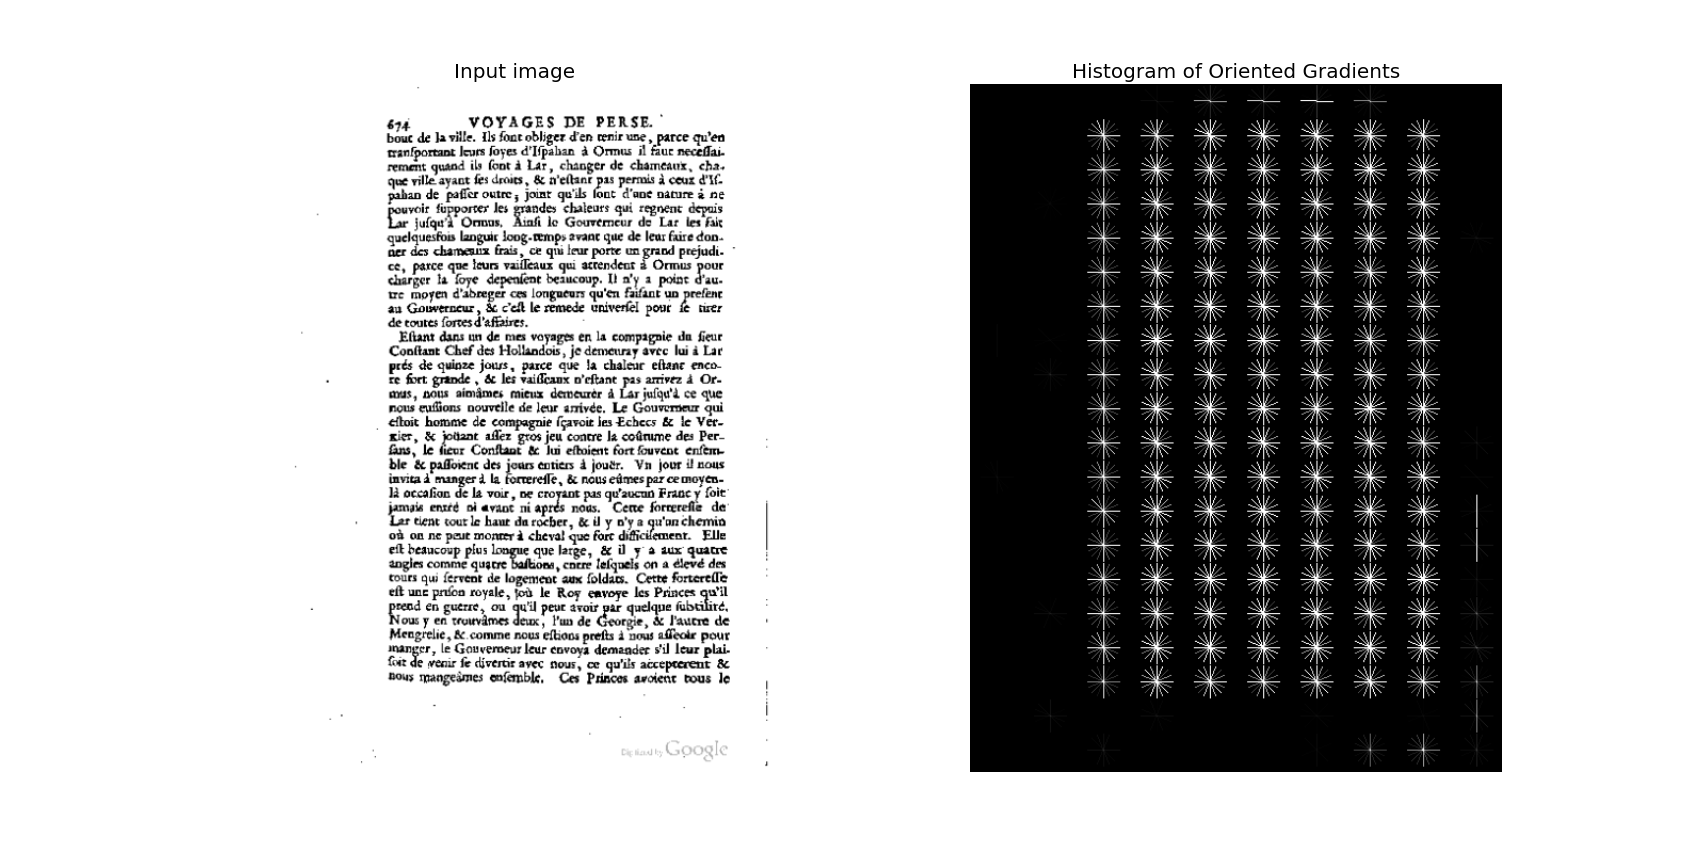
\includegraphics[trim=200px 0px 100px 0px, clip=true, width=.8\paperwidth]{resources/text1}\\
\framebreak
	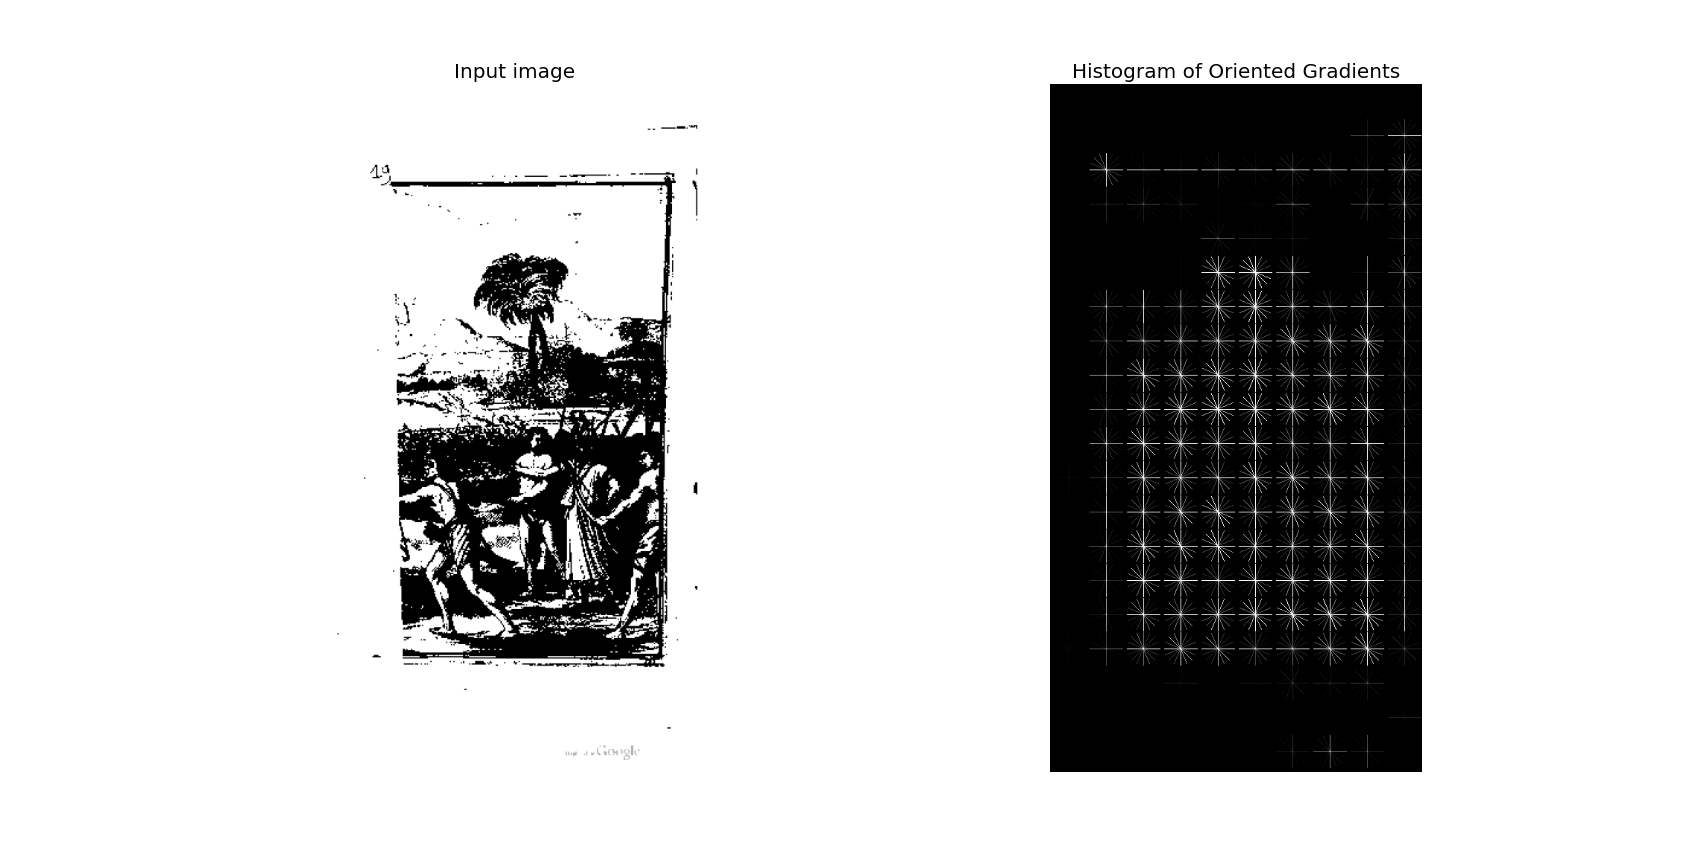
\includegraphics[trim=200px 0px 100px 0px, clip=true, width=.8\paperwidth]{resources/image1}\\
\framebreak
	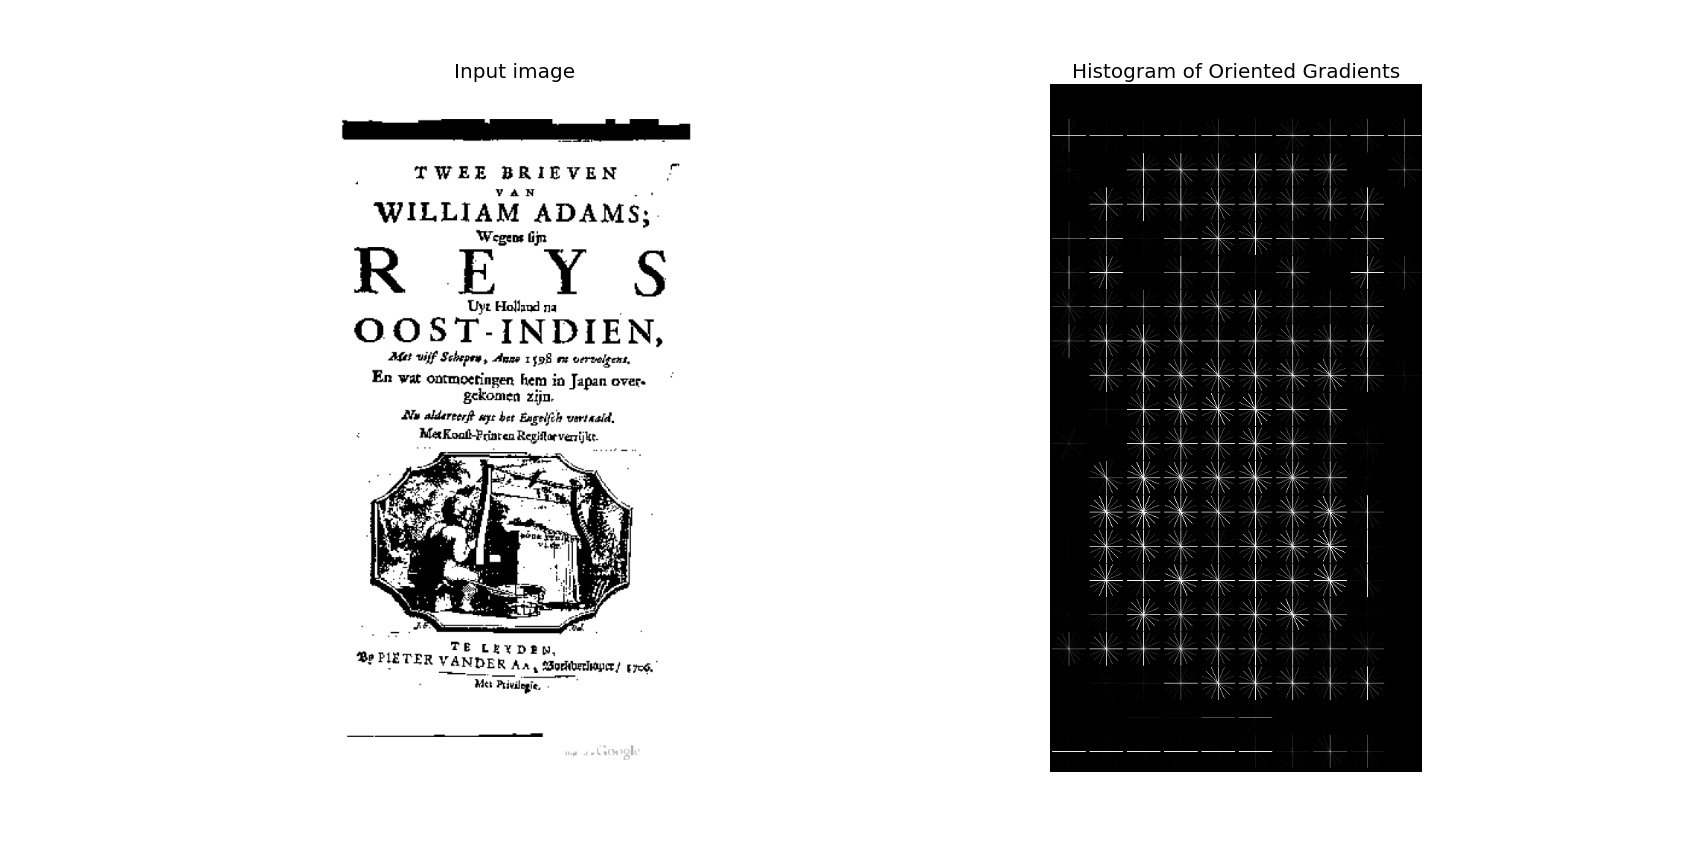
\includegraphics[trim=200px 0px 100px 0px, clip=true, width=.8\paperwidth]{resources/text_and_image1}
\end{frame}

% Explain SVM i.c.w. HOG features for pages
% Moved to introduction
% \slide{Classification using SVM}
% {
% 	\begin{itemize}
% 		\item All pages are annotated with having either ``text'', ``images'' or
% 		``nothing useful'' on it. Images get bounding boxes, which we will later
% 		use.
% 		\item Calculate 5x5 HOG features per page
% 		\item Train a Support Vector Machine (SVM) on these feature vectors and
% 		labels
% 		\item Predict whether a page contains an image based on this SVM
% 	\end{itemize}
% }

\begin{frame}
\frametitle{Test - Validation}
\begin{itemize}
\item Merge the sets of all annoated book pages into one set
\item Split this set into train set ($80\%$) and validation set($20\%$)
\item Use validation set to set parameters ($C$)
\end{itemize}


\end{frame}

\subsection{Results}
\begin{frame}
\frametitle{Results}
\begin{itemize}
\item Run the learned classifier on new books
\item Use F2-score in order to focus on recall (preprocess for annotator)
\end{itemize}
TODO: list results

\end{frame}

\subsection{Method}
\label{subsec:pageclasmethod}
\subsection{Method}
\label{subsec:pageclasmethod}
HOG \cite{dalal2005histograms} features are used to locally describe image
patches.
\todo{explain hog features here}

Using the annotated 

% \begin{frame}
% \frametitle{Features}
% Local features to capture the difference between text and images:
% 	\begin{block}{Histogram of Oriented Gradients (HOG)}
% 		HOG features contain the amount of gradients in a certain image patch.
% 	\end{block}
% 	\begin{block}{Steps for computing HOG Features\cite{dalal2005histograms}}
% 	\begin{enumerate}
% 		\item Global image normalisation
% 		\item Compute the gradient images
% 		\item Compute gradient histograms in 8 directions
% 		\item Normalise across blocks
% 		\item Flatten into a feature vector
% 	\end{enumerate}
% 	\end{block}
% \end{frame}

\todo{Describe (shortly) the train, validation and test set}

\todo{Describe learning the SVM}


\subsection{Results}
\label{subsec:pageclasresults}
\subsection{Results}
\label{subsec:pageclasresults}

In order to use the page classification as a preproccessing step for annotating
books, a page classifier would have to have a very high recall. Therefore, the
results shown in this section, are validated using the F2 score on the image
class. 

% It is my (Maartens) opinion that we should describe our parameters for HOG
% features at the same time as our parameters for the SVMs. Maybe we should even
% move this to the "results" section.
Each page was divided into 5 by 5 blocks. Because the pages
are quite alike in terms of lighting conditions\footnote{they are all scanned
similarly, and pages are mostly black on white}, each block had only 1 cell. For
calculating the HOG features, the gradients were binned into eight orientations.
This means the feature vectors for the Linear SVM have $8 \times 5 \times 5 =
200$ dimensions. 
For the SVM constant \emph{C} was validated with $10^c$, with $c = \{1 \dots
6\}$, L2 (squared hinge) loss was used and the dual problem was solved. 

\begin{table}
\centering
\begin{tabular}{l r r r}
\hline
% & \multicolumn{2}{c}{\emph{Pre-trained}} & \multicolumn{2}{c}{\emph{Direct}} \\
  & \textbf{Image} & \textbf{Text} & \textbf{Nothing} \\\hline
\textbf{Precision} & 0.600  & 0.995 & 0.970 \\
\textbf{Recall} & 0.964  & 0.921 & 0.964 \\
\textbf{F2-score} & 0.741 & 0.956 & 0.967 \\\hline
\end{tabular}
\caption{Resulting scores of the page classifier on each of the three annotated
classes.}
\label{tab:pageclasresults}
\end{table}

% Maybe this could just be in the same table as the previous tabular
\begin{table}
\centering
\begin{tabular}{l r r r}
\hline
%& \multicolumn{2}{c}{\emph{Pre-trained}} & \multicolumn{2}{c}{\emph{Direct}} \\
Real\textbackslash Predicted & \textbf{Image} & \textbf{Text} & \textbf{Nothing} \\\hline
\textbf{Image} & 271 & 9 & 1 \\
\textbf{Text} & 169 & 2074 & 9 \\
\textbf{Nothing} & 10 & 2 & 323\\
\hline
\end{tabular}
\caption{Confusion matrix of the page classifier}
\label{tab:pageclascm}
\end{table}

Table \ref{tab:pageclasresults} shows three measures of accuracy of the
classifier on the test set. As can be seen validating using the F2-score
results in a big recall, but in relatively low precision on the image
class as well. These results mean that when this classifier would be used as a
preprocessing step for annotating, about $3.6\%$ of the pages containing images
would not be annotated as such. Table \ref{tab:pageclascm} depicts the confusion
matrix.




\section{Image Localization}
\label{sec:imageloc}

\begin{frame}
\frametitle{Image Locatization}
Second step:
\begin{itemize}
\item find bounding boxes of images on new books
\item classify whether patch is an image or text patch
\item reconstruct images from patches
\end{itemize}
HOG features:
\begin{itemize}
\item 10x20 per page
\item Additionally: concatenate features, 9x19 per page
\end{itemize}
\end{frame}

\subsection{Method}
\begin{frame}
\frametitle{Conditional Random Fields}
\begin{itemize}
\item Regard image as undirected graph (labels $x_i$, patches $y_i$)
\item Decide label for $x_i$ on patch likeliness, neighborhood, and prior
\item Solver: Structural Support Vector Machine (SSVM)
\end{itemize}
$$ E(\mathbf{x}, \mathbf{y}) = h\sum_i x_i - \beta \sum_{\{i, j\}} x_i x_j
- \eta \sum_i x_i y_i $$

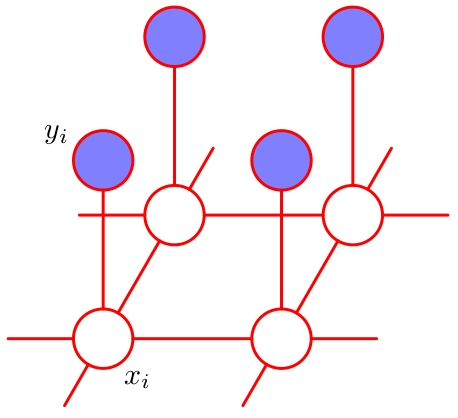
\includegraphics[width=.3\paperwidth]{resources/crf}
\end{frame}

\begin{frame}{CRF and SSVM}

\begin{itemize}
\item To solve the CRF, the energy function must be minimized.
\item For this, two types of SSVMs can be used:
\begin{itemize}
	\item N-slack SSVM
	\item One-slack SSVM
\end{itemize}
\item $\argmin \hat{y} \text{E}(x, y) + \text{loss}(\hat{y}, y) $
\item Where the loss is the \emph{Hamming} loss
\end{itemize}
\end{frame}

\begin{frame}
\frametitle{Preprocess Features Using an SVM}
\begin{itemize}
\item HOG features have 8 values
\item SSVM is harder to solve for more dimensions per feature
\item Use SVM to assign confidence score to each feature
\item Now SSVM has input of 1 dimension per feature
\end{itemize}
\end{frame}

\begin{frame}
\frametitle{Two Stage Training}
Require two stage training to prevent overfitting.
\begin{itemize}
\item Train SVM on $75\%$ of train set, and predict labels on remainder for SSVM
\item Repeat 4 times, with different splits
\item Now $100\%$ of the SSVM features is available
\item Once more: train SVM on $100\%$ of train set to obtain best model
\end{itemize}
\begin{center}
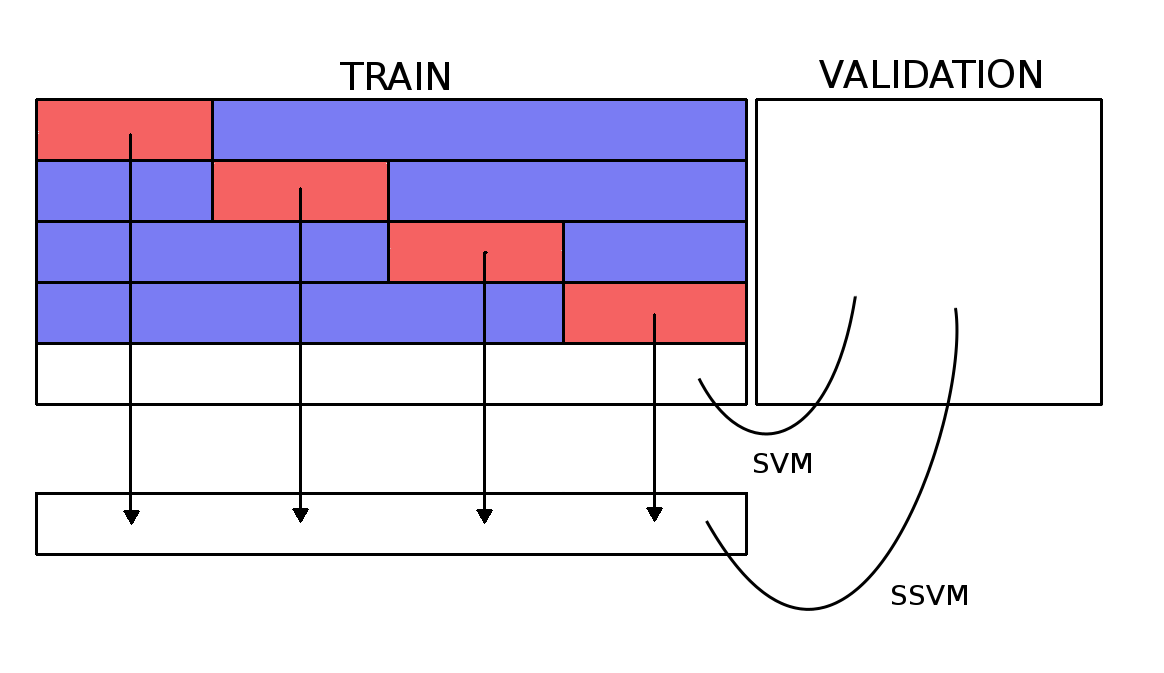
\includegraphics[width=.5\paperwidth]{resources/twostage}
\end{center}
\end{frame}

\subsection{Results}

\begin{frame}
\frametitle{Results}
insert results here
\end{frame}

\subsection{Method}
\label{subsec:imagelocmethod}
\begin{figure}
\begin{floatrow}
	\ffigbox{
		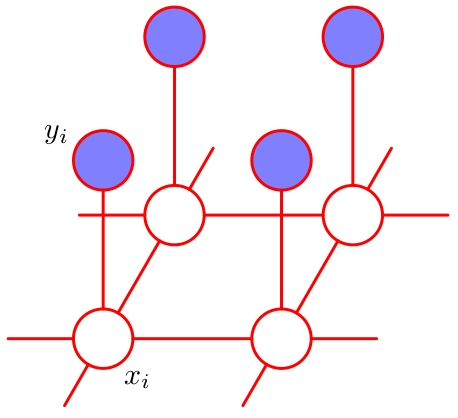
\includegraphics[width=.3\textwidth]{resources/crf}
	}{
		\caption{An undirected graph, representing the graph that was used for
		modeling our Conditional Random Field}
		\label{fig:crf}
	}
	\capbtabbox{%
		\begin{tabular}{@{\extracolsep{4pt}}l r r r r @{}}
		\hline
		 & \multicolumn{2}{c}{\emph{Pre-trained}} & \multicolumn{2}{c}{\emph{Direct}} \\
		 \cline{2-3} \cline{4-5}
		  & \textbf{Image} & \textbf{Text} & \textbf{Image} & \textbf{Text} \\
		\textbf{Precision} & 0.269 & 0.979 & 0.241 & 0.979 \\
		\textbf{Recall} & 0.743 & 0.854 &  0.750 & 0.830 \\
		\textbf{F-score} & 0.395 & 0.912 & 0.365 & 0.898 \\\hline
		\end{tabular}
	}
	{
		\caption{scores for image localization}
		\label{tab:imagelocresults}
	}
\end{floatrow}
\end{figure}
A CRF provides the labelling for an undirected graph. In this case, a grid was
used, shaped as figure \ref{fig:crf}, where $y_i$ is the percieved data for an
image patch, and $x_i$ is the label assigned to that patch by the learning
algorithm. The ultimate goal is to find the labelling for $\mathbf{x}$ that
minimizes the loss function. 

For calculating this loss function, the CRF has an energy function for each pair
$\{x_i, y_y\}$, a simple
example of which, taken from \cite{bishop2006pattern}\footnote{This example is actually
used in an example of Markov Random Fields, but this specific graph is
comparable to a CRF},  has the following form: 
\begin{equation}
E(\mathbf{x}, \mathbf{y}) = h\sum_i x_i - \beta \sum_{\{i, j\}} x_i x_j
- \eta \sum_i x_i y_i
\end{equation}
In this energy function, $\eta$ is a positive constant. The product $\eta \sum_i
x_i y_i$ will then be of a greater number when $x_i$ and $y_i$ are similar.
$\beta$ is another positive constant, which, in combination with the sum of
products $x_i x_j$ should result in higher energy when the neigbouring nodes
$x_j$ have a similar value to $x_i$. Finally $h$ is a constant that can be used
to bias the energy function to either one of the classes, for example when
dealing with an unfair distribution like ours. Various implementations of
Conditional Random Fields might use various types of energy function, but the
idea is the same.

Finding the solution with maximum energy is not trivial, since 
looping over all possible solutions and selecting the one with the highest energy
for all nodes would quickly become intractable. Therefore a solver should be
used, in this case the SSVM.

\todo{Explain the SSVM}

\todo{Explain different types of processing: preprocessed with SVM and with
either 1 or 4 HOGs per image patch}
\todo{Explain two-stage validation. Also explain why we can compare the scores
of the different SVM's (the question jan van Gemert asked)}

\subsection{Results}
\label{subsec:imagelocresults}
\subsection{Results}
\label{subsec:imagelocresults}

Again HOG features are used describe image patches. This time a more dense field
is required because from the image patches classified as \emph{image} the actual
images are to be extracted. For this purpose the page is divided into 10 by 20
blocks each with one cell. Optionally, features are concatenated to incorporate
more information from the region. This results in 9 by 19 concatenated
features: one feature, the features of the block to the right, to the bottom and
the right bottom are concatenated into one.

If the preprocessing step of the linear SVM is used, we need to be careful and
avoid over fitting by training the linear SVM on the same data as the structured
SVM is trained. Therefor, we used two stage validation learning (see figure
\ref{fig:twostage}). In two stage validation repeatedly, a different subset of
the training data is used to train the linear SVM. The resulting SVM assigns the
confidence score to rest of the training data in order to finally recreate the
whole training data, but now with confidence scores without the risk of
overfitting\footnote{Note that we do not use Platt scaling to normalize the
scores assigned by these different SVMs. Empirical results show that this does
actually hurts performance a little, even though more one-vs-all and all-vs-all
multi0class SVMs often exclude this step to safe time as well\cite{duan2005best}}.
%\todo{several SVMs and the confidence scores can be used?! Could only find:
%\cite{duan2005best} which indicates exactly the opposite}

\begin{figure}
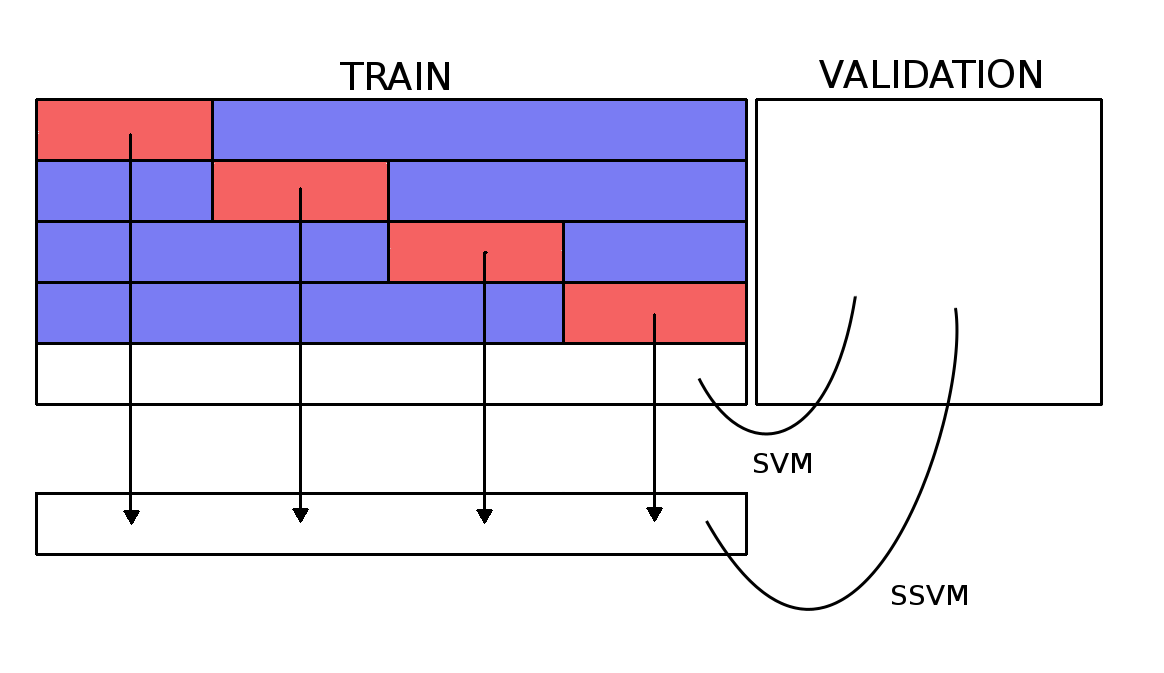
\includegraphics[width=.5\textwidth]{resources/twostage}
\caption{Visualization of two-stage validation training to generate data for the
structured SVM}
\label{fig:twostage}
\end{figure}

We experimented with 4 different settings: directly trained on the structured
SVM and pre-trained with the linear SVM, we then tested both options with the
concatenated features and with the regular features. The same division for the
train, validation and test set has been used as in section \ref{sec:pageclas}.
Tables \ref{tab:imageloccm} and \ref{tab:imagelocresults} show the results for
these settings. The `SVM Only' columns show the results of the
linear SVM for classifying single features. All scores are calculated per
feature. The true labels are based on the annotated data: whether their centre
is inside or outside a bounding box.

First, the results for the single HOG features in table \ref{tab:imageloccm}.
The extremely low precision indicates that these single HOG features are not
indicative if an image patch belongs to an image or text. Presumably, this
large error propagates through to the pre-trained setting, resulting in a low
recall for image patches there as well. The directly trained SVM was able to
achieve much better results.

\begin{table}
\centering
% Extra colsep creates fancy lines
\begin{tabular}{@{\extracolsep{4pt}}l r r r r r r @{}}
\hline
& \multicolumn{2}{c}{\emph{SVM only}} & \multicolumn{2}{c}{\emph{Pre-trained}} & \multicolumn{2}{c}{\emph{Direct}}
\\\cline{2-3}\cline{4-5}\cline{6-7}
& \textbf{Image} & \textbf{Text} & \textbf{Image} & \textbf{Text} & \textbf{Image} & \textbf{Text} \\
%\textbf{Precision} & 0.099 & 0.973 & 0.271 & 0.979 & 0.271 & 0.979 \\
%\textbf{Recall} & 0.736 & 0.585 & 0.700 & 0.884 & 0.700 & 0.884 \\
%\textbf{F-score} & 0.174 & 0.730 & 0.391 & 0.929 & 0.391 & 0.929\\\hline
%%% NOOOOOO wrooonnggg!
\textbf{Precision} & 0.099 & 0.973 & 0.703 & 0.944 & 0.271 & 0.979 \\
\textbf{Recall}    & 0.736 & 0.585 & 0.040 & 0.999 & 0.700 & 0.884 \\
\textbf{F-score}   & 0.174 & 0.730 & 0.075 & 0.970 & 0.391 & 0.929\\\hline
\end{tabular}
\caption{Results for image localization with single features}
\label{tab:imageloccm}
\end{table}

Second, the results for the concatenated features in table
\ref{tab:imagelocresults}. The concatenated features seem to convey more
information about the image patch, as indicated by the rise in precision and
recall for the linear SVM. As a result, the score difference 
in the pre-trained and the directly trained experiments are small, but favor the
pre-trained setting slightly.

\begin{table}
\centering
\begin{tabular}{@{\extracolsep{4pt}}l r r r r r r @{}}
\hline
 & \multicolumn{2}{c}{\emph{SVM Only}}  & \multicolumn{2}{c}{\emph{Pre-trained}} & \multicolumn{2}{c}{\emph{Direct}} \\
 \cline{2-3} \cline{4-5} \cline{6-7}
  & \textbf{Image} & \textbf{Text} & \textbf{Image} & \textbf{Text} & \textbf{Image} & \textbf{Text} \\
\textbf{Precision} & 0.154 & 0.973 & 0.269 & 0.979 & 0.241 & 0.979 \\
\textbf{Recall} & 0.732 & 0.709 & 0.743 & 0.854 &  0.750 & 0.830 \\
\textbf{F-score} & 0.254 & 0.820 & 0.395 & 0.912 & 0.365 & 0.898 \\\hline
\end{tabular}
\caption{scores for image localization with concatenated features}
\label{tab:imagelocresults}
\end{table}

We can deduce that the CRF, solved by the structured SVM improves performance
significantly.


%\begin{table}
%\centering
%% Extra colsep creates fancy lines
%\begin{tabular}{@{\extracolsep{4pt}}l r r r r r r @{}}
%\hline
%& \multicolumn{2}{c}{\emph{SVM only}} & \multicolumn{2}{c}{\emph{Pre-trained}} & \multicolumn{2}{c}{\emph{Direct}}
%\\\cline{2-3}\cline{4-5}\cline{6-7}
%Real\textbackslash Predicted & \textbf{Image} & \textbf{Text} & \textbf{Image} & \textbf{Text} & \textbf{Image} & \textbf{Text} \\
%\textbf{Image} & 24160 & 8844 & 524523 & 58481 & 524759 & 58245 \\
%\textbf{Text} & 133044 & 324380 & 566567 & 5390857 & 577927 & 5379497 \\\hline
%\end{tabular}
%\caption{Confusion Matrix for image localization with concatenated features}
%\label{tab:imageloccm}
%\end{table}


%\begin{table}
%\centering
%% Extra colsep creates fancy lines
%\begin{tabular}{@{\extracolsep{4pt}}l r r r r r r @{}}
%\hline
%& \multicolumn{2}{c}{\emph{SVM only}} & \multicolumn{2}{c}{\emph{Pre-trained}} & \multicolumn{2}{c}{\emph{Direct}}
%\\\cline{2-3}\cline{4-5}\cline{6-7}
%Real\textbackslash Predicted & \textbf{Image} & \textbf{Text} & \textbf{Image} & \textbf{Text} & \textbf{Image} & \textbf{Text} \\
%\textbf{Image} & 24565 & 8800 &  523370 &  59995 & 523370 & 59995 \\
%\textbf{Text} & 224329 & 315906 &  562795 &  5477440 & 562795 & 5477440\\\hline
%\end{tabular}
%\caption{Confusion Matrix for image localization with concatenated features}
%\label{tab:imageloccm}
%\end{table}

%\todo{Explain results, mention that the difference between Pre-trained and
%not pre-trained is bigger with more discriminative features (2x2 HOG in stead of
%1)}

\todo{Visualisations of the results (if possible). Thomas mentioned showing some
pages with the classification as a colored overlay, or a map of the labels under
the page}


\section{Discussion \& Conclusion}
\label{sec:discussionconclusion}
\section{Discussion \& Future Work}% \& Conclusion}
\label{sec:discussionconclusion}

%\todo{Say we didn't use OCR and maybe why. Also name stroke transform}
We have laid the ground work to segmentate images from text in old books. An
annotator was built which can be extended by implementing a filter
based on the results of the page classifier SVM of section \ref{sec:pageclas}.

Furthermore we have shown that a conditional random field with a 1-slack
structured SVM improves upon the results of a linear SVM that ignores the
neighborhood of its labels.

We have deliberately not chosen to implement existing techniques such as OCR to
recognize text as a feature for image patches, and a sliding window approach to
segmentate images. While this may have hindered performance, we can sure tell
that we have learned more.

For future work the poor performance of the HOG features need to be
investigated. Different parameters in the feature extraction phase, or even
different features all together, might result in more descriptive features.
Additionally, OCR for the features and a sliding window approach could be tried
out. Finally the Hamming loss that is used in solving the structured SVM
could be replaced with a loss that incorporates the rectangle shape of the
bounding boxes for the images.



\bibliographystyle{abbrv}
\bibliography{references}
\end{document}
% vim: set spell :
